\documentclass[../../../topic_statistics]{subfiles}

\begin{document}

\sectionline
\section{相対度数と確率}

ここで、\keyword{相対度数}は、全体において各階級の値が現れる割合を表していた。

この割合は、無作為抽出のもとでは「全体の中である階級値のデータが現れる\keyword{確率}」と捉えることができる。

\br

たとえば、$173$cm台という階級の相対度数が$0.25$だったとする。

このとき、抽出に偏りがないことから、$173$cm台という値が母集団全体の$25\%$を占めているといえるので、母集団全体から標本を取り出したときに$173$cm台という値が得られる確率も$25\%$となる。

\begin{emphabox}
  \begin{spacebox}
    \begin{center}
      無作為抽出では、相対度数は確率を表す
    \end{center}
  \end{spacebox}
\end{emphabox}

実際、相対度数$\dfrac{f_i}{N}$の合計は$1$となるので、確率の定義も満たしている。
\begin{equation*}
  \sum_{i=1}^N \frac{f_i}{N} = \frac{1}{N} \sum_{i=1}^N f_i = \frac{1}{N}\cdot N = 1
\end{equation*}

\sectionline
\section{標本と確率変数}

ここで、$X$という値が得られる確率を関数に見立てて、次のように表そう。
\begin{equation*}
  P(X)
\end{equation*}

$173$cm台という値が得られる確率は、次のように書ける。
\begin{equation*}
  P(X = 173\text{cm台}) = 0.25
\end{equation*}

この関数の引数となる変数$X$を、\keyword{確率変数}という。

\br

確率変数は、「結果を言い当てることはできないが、とりうる値とその値が出る確率が決まっている」ものをいう。

\begin{definition}{確率変数}
  取りうる値すべてに対して確率を考えることができるような変数
\end{definition}

ここで、「$173$cm台という値が得られた」ということは、「取り出した標本が$173$cm台だった」ということなので、$X$は\keyword{標本}である。

\begin{emphabox}
  \begin{spacebox}
    \begin{center}
      無作為抽出では、標本は確率変数とみなせる
    \end{center}
  \end{spacebox}
\end{emphabox}

\sectionline
\section{母集団の度数分布と確率分布}

この$P(X)$は、各値$X$がどれくらいの確率で出るかを表す関数といえる。

\br

$X$の取りうる値それぞれに対して確率を割り振り、すべての確率を合計すると$1$となる。

$P(X)$は、この確率の割り振り方、すなわち全確率$1$が確率変数$X$の取りうる値にどのように分布しているかを表しているため、$X$の\keyword{確率分布}と呼ばれる。

\br

また、母集団のある階級の相対度数は、その母集団から無作為抽出された標本$X$がその階級に属する確率$P(X)$を表していた。

\begin{emphabox}
  \begin{spacebox}
    \begin{center}
      無作為抽出では、母集団の度数分布は標本の確率分布となる
    \end{center}
  \end{spacebox}
\end{emphabox}

\sectionline
\section{連続型確率分布}

階級幅を横幅、相対度数を高さとする棒グラフ(ヒストグラム)を作成すると、これはそのまま標本$X$の確率分布$P(X)$を表すグラフとなる。

\br

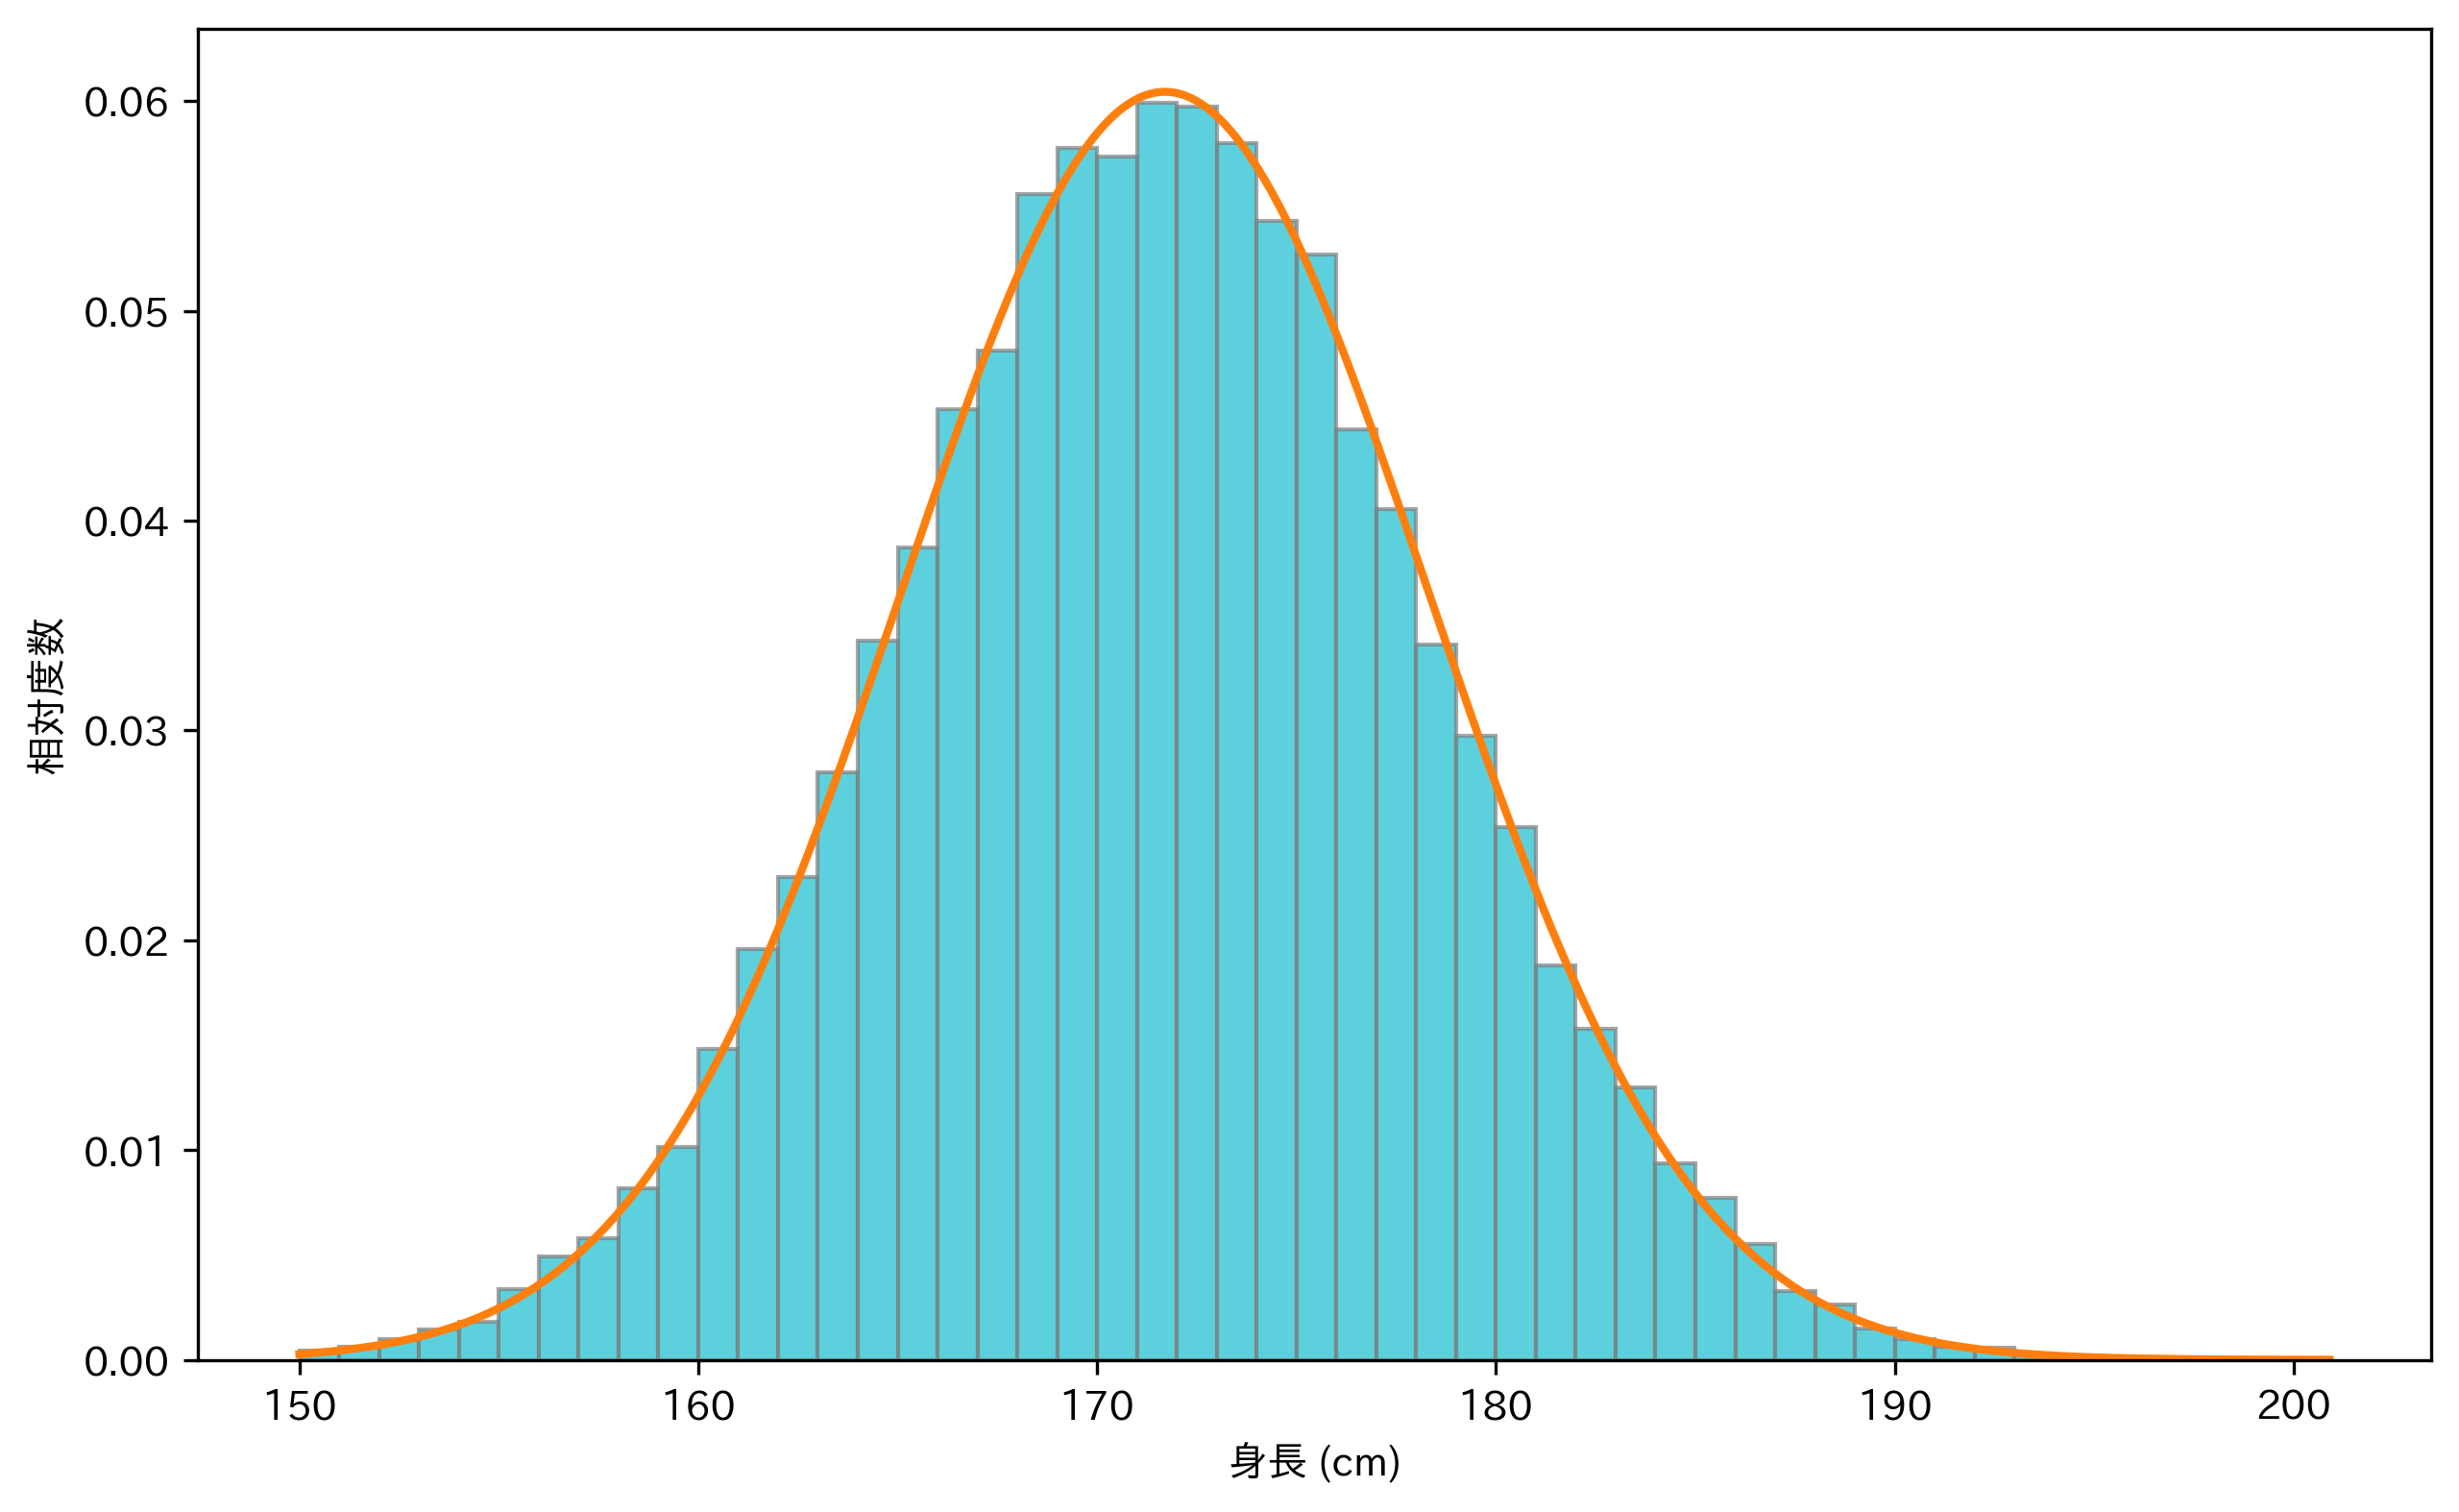
\includegraphics[width=0.95\linewidth]{./python/sampling-height_discrete.png}

\br

しかし、たとえば$173$cm台を表す棒だけでは、$173.1$cmの人が何人いて、$173.5$cmの人が何人いたのかなど、その間の分布はわからない。

\br

そこで、棒グラフの幅(階級幅)をどんどん細かくしていくことで、$173.8\dots$cmといった実際の身長に近い値(実数値)をとる確率の分布を考えることはできないだろうか?

\br

階級幅を無限に細かく分割した場合、それぞれの棒は幅が限りなく$0$に近い「線」となる。

この線の高さを結んでいくと、次のようなグラフが浮かび上がるだろう。

\br

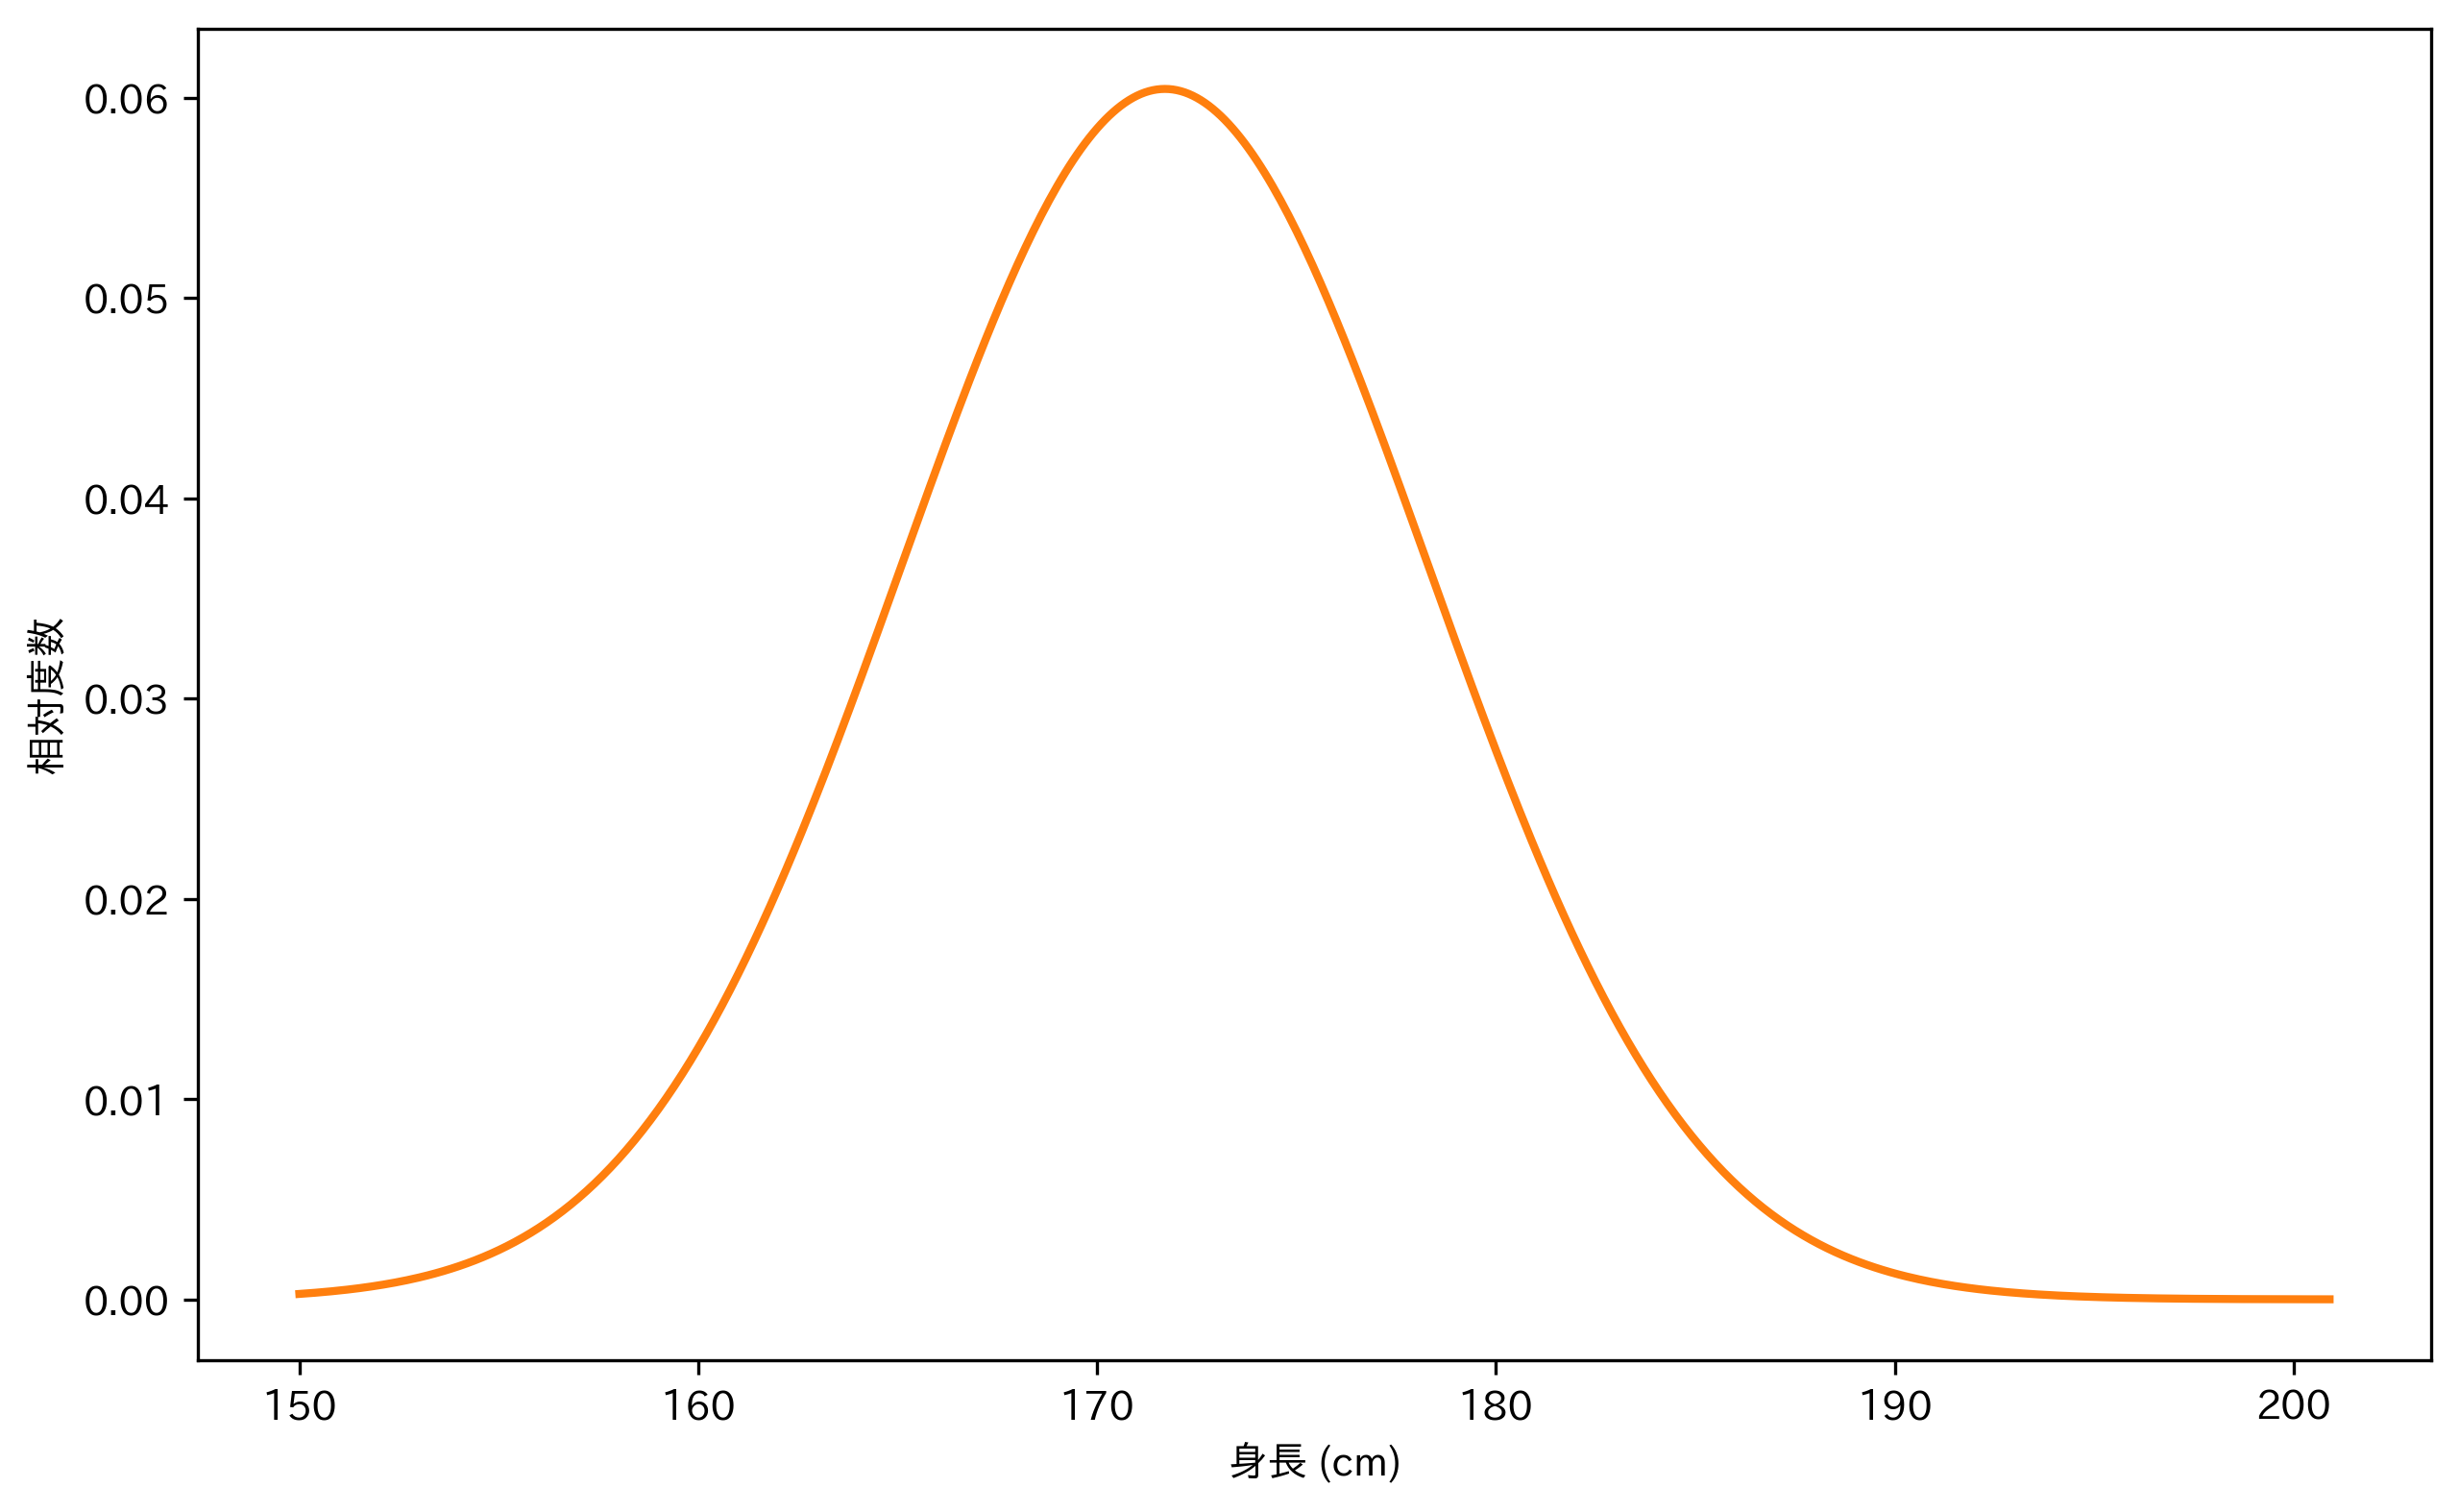
\includegraphics[width=0.95\linewidth]{./python/sampling-height_continuous.png}

\br

しかし、階級幅を小さくしていくと、各階級に含まれるデータの数(度数)はどんどん少なくなっていく。
これは、相対度数(確率)の式$\dfrac{f_i}{N}$でいえば、度数$f_i$がどんどん小さくなっていくことに相当する。
\begin{equation*}
  \lim_{f_i \to 0} \frac{f_i}{N} = 0
\end{equation*}

このように、連続的なデータ(実数値をとるデータ)では、完全に一致する値(特定の1点)が出る確率は$0$となってしまう。

だから「173cm台」すなわち「173cm以上174cm未満」といった区間に対して確率を考えていたのである。

\br

確率変数$X$が実数値をとるような確率分布は、\keyword{連続型確率分布}と呼ばれる。

連続型確率分布では、「ある区間に入る確率」を考えるしかない。

\br

$P(X = 173\text{cm台}) = 0.25$という確率の式は、区間に入る確率として、次のように書き換えられる。
\begin{equation*}
  P(173 \leq X < 174) = 0.25
\end{equation*}

\subsection{確率密度関数}

グラフを見ると、たとえば$172.0$cmというデータが得られる確率(相対度数)と、$172.5$cmというデータが得られる確率は、ほぼ同じだといえる。

\br

このように、区間幅$\Delta x$が十分に小さいとき、$X = x$での確率と、$X = x + \Delta x$での確率はほぼ同じになる。

そこで、幅$\Delta x$の棒を立てたとき、その棒($\Delta x$は微小なのでほとんど線に見える)の高さは、ほぼ1点$X = x$での確率と見なすことができる。

\br

ほぼ1点$X = x$での確率を高さ$f(x)$とみなせるなら、そこに区間幅$\Delta x$をかけることで、区間に対する確率が求められる。
\begin{equation*}
  P(x \leq X < x + \Delta x) = f(x) \Delta x
\end{equation*}

\br

幅$\Delta x$の棒を、区間$[a, b)$を埋め尽くすように並べたとしよう。

しかし、区間$[a, b)$内で確率が変化しないとは限らないので、それぞれの棒の高さ$f(x)$は$X$の値$x$によって異なる。

\br

そこで、「$x$を変化させながら$f(x)\Delta x$を足し合わせる」という演算が必要になる。

このような演算は、\keyword{定積分}として定義される。

\begin{equation*}
  P(a \leq X < b) = \int_a^b f(x) dx
\end{equation*}

\br

たとえば、$170$cm以上$180$cm未満の区間に対する確率$P(170 \leq X < 180)$は、次のピングの領域の面積として求められる。

\br

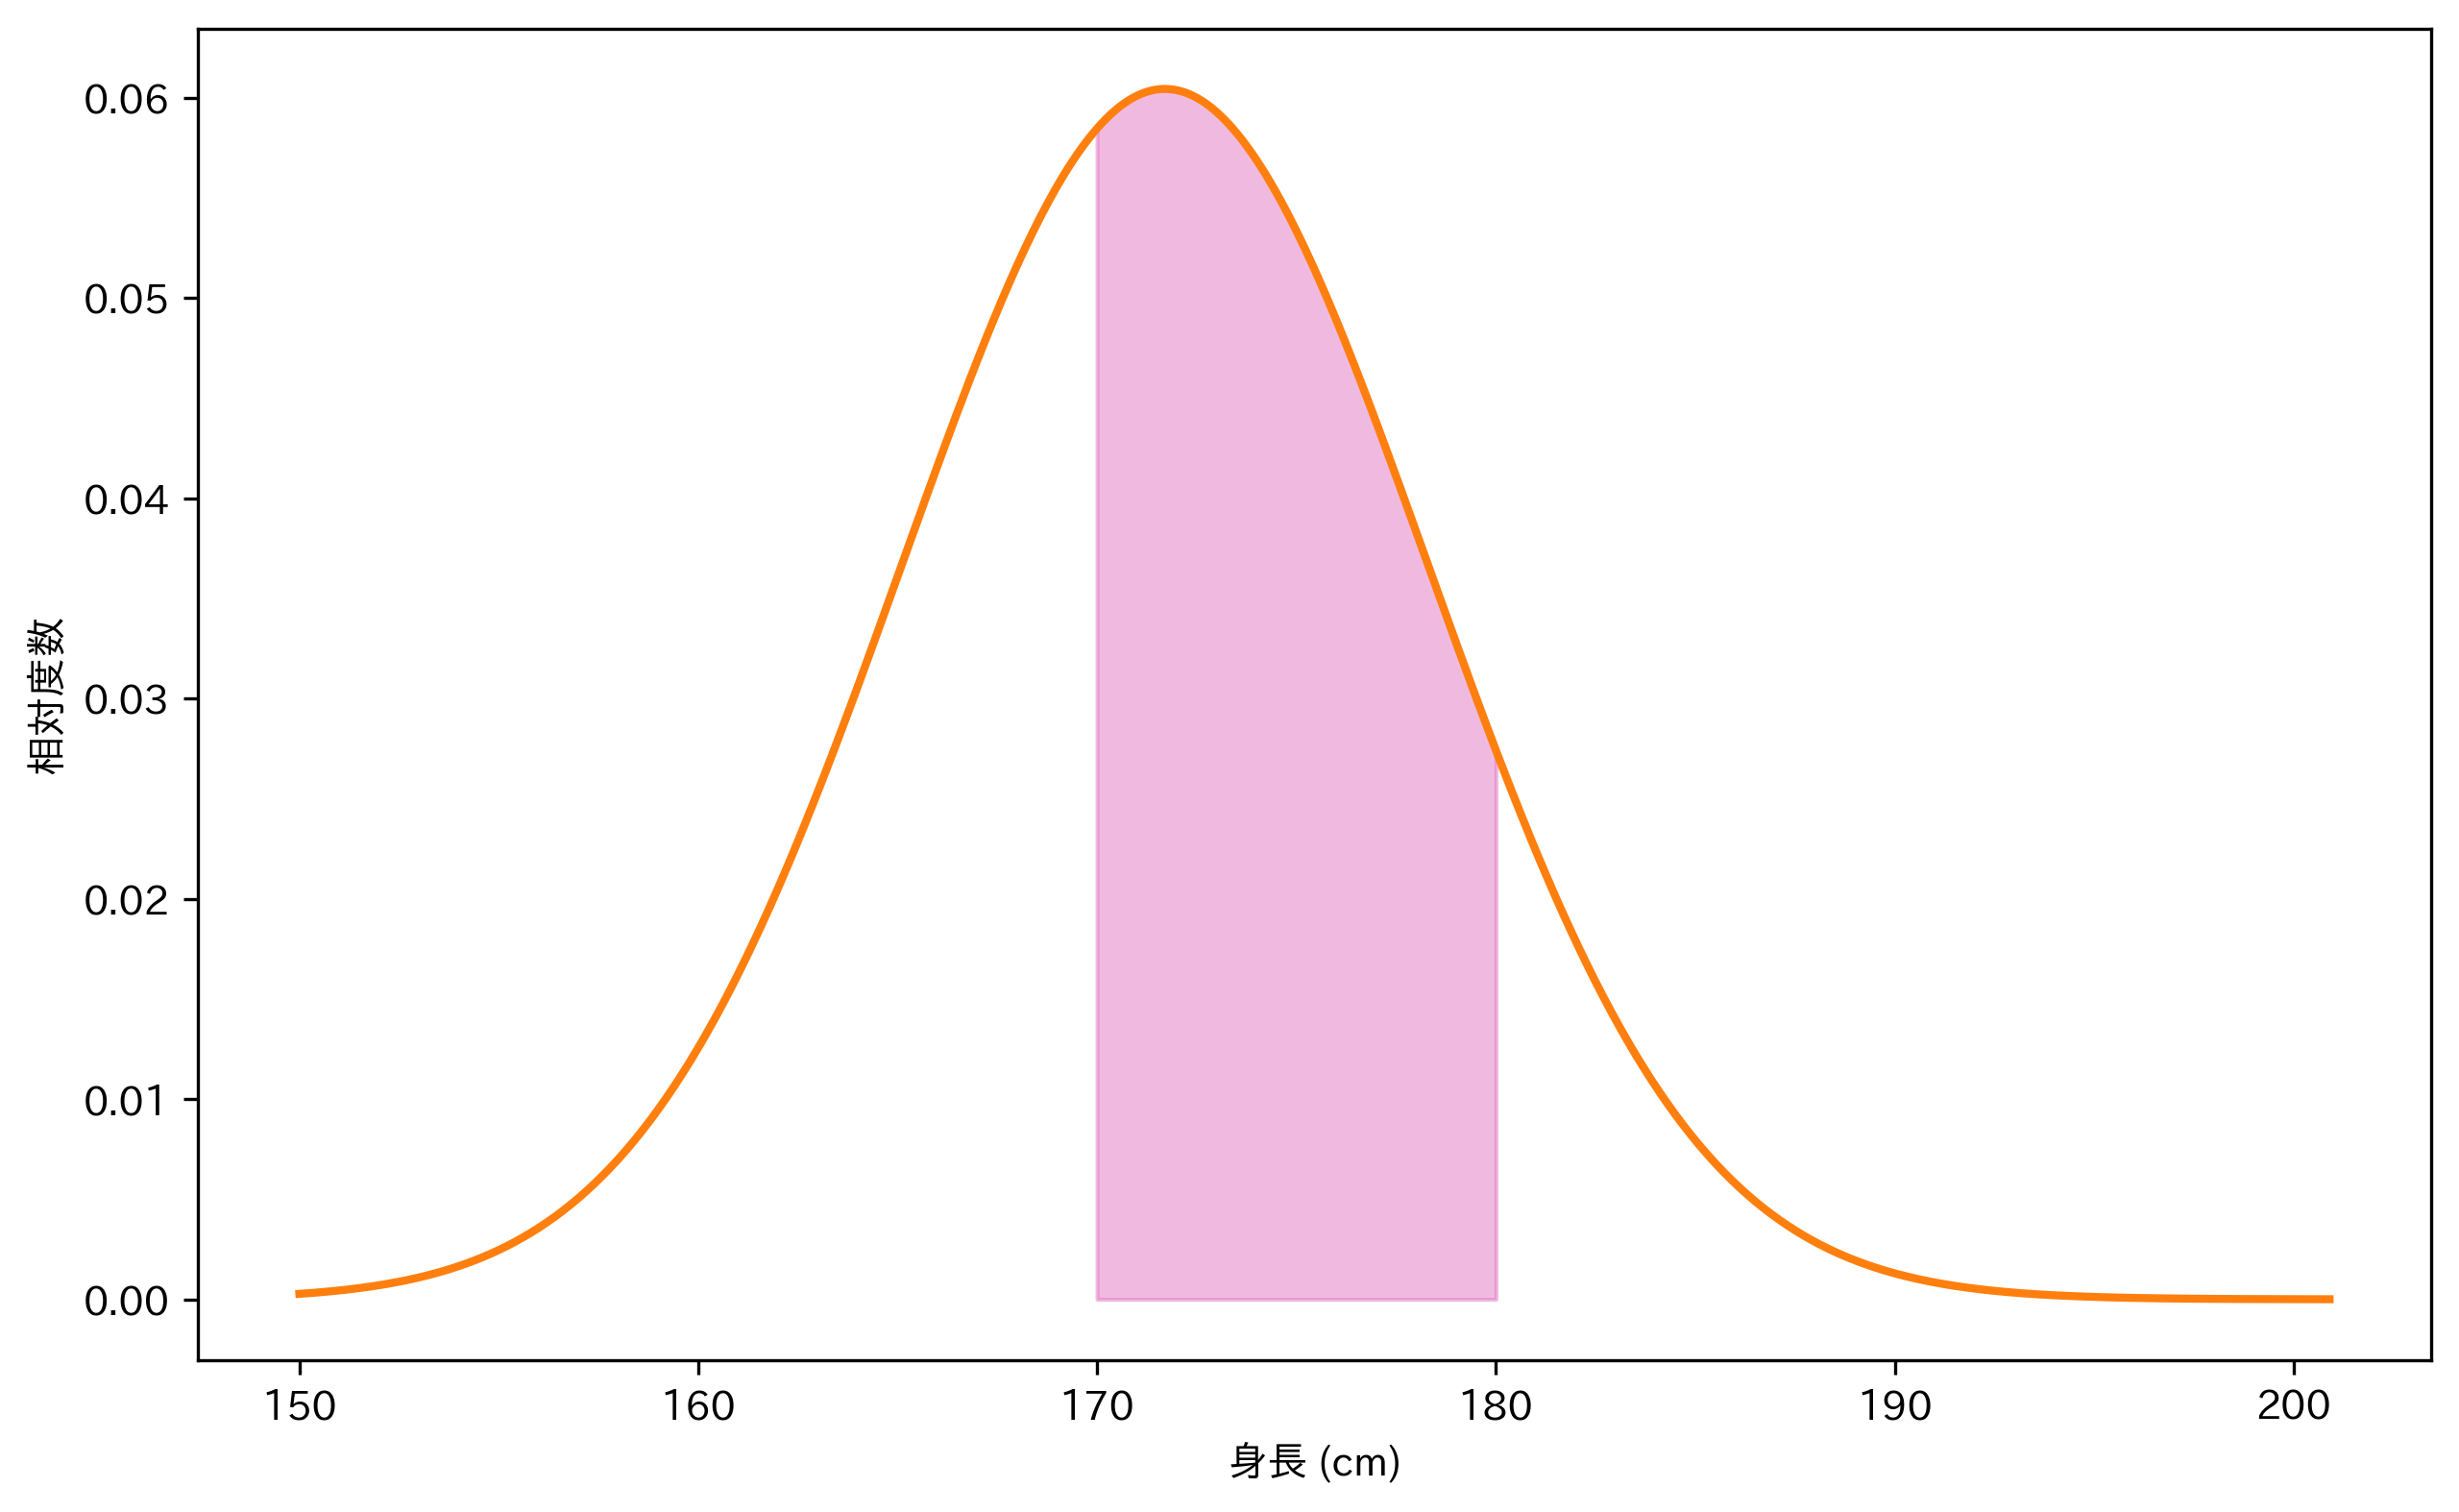
\includegraphics[width=0.95\linewidth]{./python/sampling-height_probability.png}

\br

このように、連続型確率分布では、定積分(面積)によって区間に対する確率を定義する。

積分すると確率が求まるような関数$f(x)$を\keywordJE{確率密度関数}{PDF: probability density function}と呼ぶ。

\br

確率の総和は$1$であるから、全区間に対する確率密度関数の定積分(全面積)は$1$となる必要がある。
確率密度関数は、次の性質を満たすものとして定義される。
\begin{equation*}
  \int_{-\infty}^{\infty} f(x) dx = 1, \quad f(x) \geq 0
\end{equation*}

\sectionline
\section{離散型確率分布}

$X$が実数値をとる連続型確率分布に対して、$X$が整数などの離散値をとる場合の確率分布を\keyword{離散型確率分布}と呼ぶ。

離散値とは、たとえばサイコロの目$1, 2, 3, 4, 5, 6$のように、値が飛び飛びで連続していないものをいう。

\br

サイコロの目を確率変数$X$とすると、$X$が$1$の目を出す確率は、次のように表される。
\begin{equation*}
  P(X = 1) = \frac{1}{6}
\end{equation*}

\subsection{確率質量関数}

一般に、確率変数$X$が値$x_i$をとる確率が次のように表されるとき、
\begin{equation*}
  P(X = x_i) = f(x_i)
\end{equation*}
ここで現れた$f(x)$は確率変数$X$の\keywordJE{確率質量関数}{PMF: probability mass function}と呼ばれる。

\end{document}
